%
% main.tex -- Paper zum Thema Audio-Kompression mit Daubechies-Wavelets
%
% (c) 2019 Hochschule Rapperswil
%
\chapter{Audio-Komprimierung mit Daubechies Wavelets\label{chapter:compress}}
\lhead{Audio-Komprimierung mit Daubechies Wavelets}
\begin{refsection}
\chapterauthor{Julian Bärtschi}

\section{Audio-Komprimierung}
\rhead{Vorwort}
Die Menge an produzierten Daten nimmt jährlich rasant zu.
Immer höher auflösende Bild-/ Video und Audiodaten spielen dabei eine zentrale Rolle.
Um den Berg an Daten im Griff zu behalten, muss der Datenkomprimierung (lat.~comprimere, `zusammendrücken') eine grosse Bedeutung beigemessen werden. 

Das Ziel der Datenkomprimierung ist es, die vorhandenen Daten so zu verdichten, dass der Speicherbedarf möglichst reduziert werden kann.
Es sollen für die Speicherung, wie auch für die Übertragung der Daten möglichst wenig Ressourcen benötigt werden.
Grundsätzlich unterscheidet man dabei zwischen verlustbehafteter und verlustfreier Kompression.

Diese Arbeit wird auf Audiodaten beschränkt.
Dabei ist das Ziel nicht etwa die Entwicklung eines Kompressionsalgorithmus sondern das Aufzeigen von Möglichkeiten der Komprimierung mit Hilfe von Wavelets.

\subsection{Verlustfreie Komprimierung}
Bei der verlustfreien Komprimierung wird gewährleistet, dass die Originaldaten exakt aus den komprimierten Daten wiederhergestellt werden können.
Es wird die Tatsache ausgenutzt, dass gewisse Daten redundant vorkommen. 
Deshalb spricht man auch von Redundanzreduktion.

Verlustfreie Komprimierung findet breite Anwendung.
Insbesondere bei Datenarchivierung sollen die Originaldaten exakt erhalten bleiben und darum wird häufig eine solche Kompressionstechnik verwendet.
Namhafte Beispiele von verlustfreier Komprimierung sind beispielsweise das ZIP-Dateiformat, die Portable Network Graphics (PNG) oder im Bezug auf Audiodaten der Free Lossless Audio Codec (FLAC).
Mit heutigen Verfahren können Kompressionsraten von 25 bis 70 Prozent erreicht werden.

\subsection{Verlustbehaftete Komprimierung}
Bei der verlustbehafteten Komprimierung soll nur der nötige Teil der Originaldaten erhalten bleiben.
Das hat zur Folge, dass die Originaldaten nicht mehr exakt wiederhergestellt werden können. 
Somit ist sie nicht mehr umkehrbar.
Man kann unnötige Daten entfernen und somit die Datenmenge reduzieren.
Deshalb spricht man auch von Irrelevanzreduktion.
Um zu entscheiden, welche Teile wichtig und welche entbehrlich sind, wird auf die menschliche Wahrnehmung geachtet.
Die verlustbehaftete Komprimierung wird insbesondere für Multimedia-Daten häufig verwendent.
Weil die menschliche Sinneswahrnemung nicht alle Frequenzen und Töne gleich gut aufnimmt, können gewisse Bereiche weggelassen werden.
Mehr dazu im nächsten Kapitel.

Mit der verlustbehafteten Kompression können sehr hohe Kompressionsraten erreicht werden, welche aber stets mit einer Qualitätseinbusse kommen.
Diesen Abtausch von hoher Kompression mit schlechter Qualität gilt es abzuschätzen.

\section{Psychoakustik}
\rhead{Psychoakustik}
Das menschliche Gehör verarbeitet Schallwellen nicht einfach wie ein Mikrofon.
Ein Schallereignis kann nach diversen psychoakustischen Grössen beurteilt werden.
Lautheit, Schärfe, Tonheit, Rauhigkeit und Schwankungsstärke sind dabei wichtige Parameter.
Ausserdem spielen Tonhaltigkeit und Impulshaltigkeit eine weitere Rolle.
Auf die erwähnten Parameter wird hier nicht weiter eingegangen.

\begin{figure}[h]
	\centering
	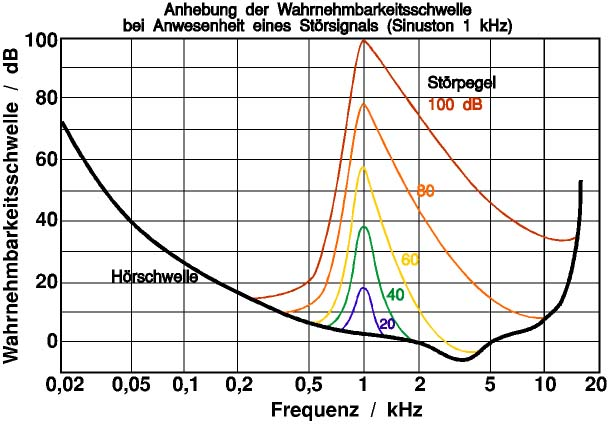
\includegraphics[width=0.6\linewidth]{papers/compress/Bilder/Akustik_Mithoerschwelle2}
	\caption{Wahrnehmbarkeit von Schallsignalen bei Anwesenheit von Störsignalen \cite{skript:Akustik2}}
	\label{fig: Wahrnehmbarkeitsschwelle}
\end{figure}

In \autoref{fig: Wahrnehmbarkeitsschwelle} Dargestellt ist ein Modell der Wahrnehmbarkeitsschwelle eines menschlichen Gehörs.
Bei einem vorhandenen Störsignal, hier $1\,\text{kHz}$, wird diese Schwelle merklich angehoben.
Auch zeitlich werden leise Töne kurz vor und nach einem lauten Ton verdeckt.

Nun folgt die Überlegung, dass jene Daten die nicht wahrnehmbar sind (unter der Schwelle) redundant sind und weggelassen werden können.
Dies suggeriert grosses Potential für die verlustbehaftete Komprimierung.

\section{Multiskalenanalyse}

\rhead{}
\section{Schlussfolgerung}
\rhead{Schlussfolgerung}

\printbibliography[heading=subbibliography]
\end{refsection}
